\documentclass[12pt,a4paper]{article}

\usepackage{a4wide}
\usepackage{graphicx}
\usepackage{amsmath,amssymb}
\usepackage{ae,aecompl}
\usepackage{amsthm}

%\pagestyle{empty}
\setlength{\parindent}{0pt}
\renewcommand{\labelenumi}{\alph{enumi})}
\renewcommand{\labelenumii}{\roman{enumii})}

% Neutrino oscillation channels
\newcommand{\ee}{\ensuremath{\nu_e \rightarrow \nu_e}}
\newcommand{\emu}{\ensuremath{\nu_e \rightarrow \nu_\mu}}
\newcommand{\etau}{\ensuremath{\nu_e \rightarrow \nu_\tau}}
\newcommand{\mue}{\ensuremath{\nu_\mu \rightarrow \nu_e}}
\newcommand{\mumu}{\ensuremath{\nu_\mu \rightarrow \nu_\mu}}
\newcommand{\mutau}{\ensuremath{\nu_\mu \rightarrow \nu_\tau}}
\newcommand{\taue}{\ensuremath{\nu_\tau \rightarrow \nu_e}}
\newcommand{\taumu}{\ensuremath{\nu_\tau \rightarrow \nu_\mu}}
\newcommand{\tautau}{\ensuremath{\nu_\tau \rightarrow \nu_\tau}}

% Neutrino oscillation parameters
\newcommand{\sthsol}{\ensuremath{\sin^2 2\theta_{12}}}     % Mixing angles
\newcommand{\sthchooz}{\ensuremath{\sin^2 2\theta_{13}}}
\newcommand{\sthatm}{\ensuremath{\sin^2 2\theta_{23}}}
\newcommand{\sthtf}{\ensuremath{\sin^2 2\theta_{2f}}}
\newcommand{\ldm}{\ensuremath{{\Delta m_{31}^2}}}          % Mass squared differences
\newcommand{\sdm}{\ensuremath{{\Delta m_{21}^2}}}

% Important neutrino experiments
\newcommand{\TtoK}{{\sffamily T2K}}

% Miscellaneous commands
\newcommand{\aufg}[2]{\vspace{4mm}{\bf\underline{Task #1:} {#2}} \vspace{3mm}}

% Environment for API reference entries
\newtheoremstyle{dotless}{}{}{\itshape}{}{\bfseries}{}{0cm}{}
\theoremstyle{dotless}
\newtheorem*{function}{}

\begin{document}
\vspace*{-3cm}
\begin{center}
{\large\bf GLoBES Tutorial: Implementing LBNE}\\[0.3cm]
GLoBES mini-workshop at Fermilab
\end{center}
\vspace*{2mm}

Joachim Kopp \hfill May 13, 2010

\bigskip
\hrule
\vspace*{4mm}

{\small
In this tutorial, we will implement LBNE (with a Water Cherenkov detector) in
GLoBES, starting from the existing AEDL (Abstract Experiment Definition
Language) file for NOvA. We will see how fluxes, efficiencies, smearing
matrices, etc.\ taken from Monte Carlo simulation can be used as input for
GLoBES. In the second part, we will discuss strategies for reliably finding
degenerate solutions in parameter space.
}


% ----------------------------------------------------------------------------
\section*{Part 1: An AEDL file for LBNE}
% ----------------------------------------------------------------------------

\aufg{1}{Warm-up: Familiarize yourself with the NOvA simulation}

Look at the file NOvA.glb: The first part defines the properties of the beam;
the spectrum is read from two external files {\tt NOvAplus.dat} and {\tt
NOvAminus.dat}. Below, we define the target mass, the binning used in the
analysis, and the baseline. The energy resolution function has the simple form
$\sigma_E = 0.1 \sqrt{E/\text{GeV}}$~GeV for $\nu_e$ and $\sigma_E = 0.05
\sqrt{E/\text{GeV}}$~GeV for $\nu_\mu$. Next comes the definition of the
various CC and NC oscillation channels, which are finally combined in
\emph{rules}, i.e.\ realistic event samples consisting of signal and background
contributions and having systematic uncertainties (normalization and spectral
tilt) associated with them.

Compile ({\tt make}) and run the program {\tt th13delta} to compute the
$\theta_{13}$ and $\delta_{CP}$ sensitivity of NOvA.%
\footnote{Note that, to speed things up, this program does not take into
account all parameter correlations and should therefore not be used for real
production runs unless appropriate modifications are made.} You can plot the
output of {\tt th13delta} using gnuplot (call the script {\tt
./th13delta.gnuplot}) or your favorite plotting program.

Familiarize yourself with the source code {\tt th13delta.c}, which
illustrates the basic structure of all GLoBES application programs:
After initialization of the library and definition of the true parameter
values and external priors, the code computes the ``true'' event rates
and then performs a $\chi^2$ fit. For each test value in the $\theta_{13}$-$\delta_{CP}$
plane, it computes the corresponding $\chi^2$, marginalizing over (some of) the other
oscillation parameters, as specified by the ``projection'' object
{\tt th13delta\_projection}.


\aufg{2}{Implenting the basic parameters of LBNE}

Let us now begin to implement LBNE. While modifying the AEDL files, you can use
the command {\tt globes LBNE.glb} to see the predicted total event rates for
each rule.  (Use {\tt globes -?} for a full list of command line options.)

For simplicity, we will only implement the case where the target is operated in
neutrino mode.  Therefore, copy {\tt NOvA.glb} to a new file {\tt LBNE.glb},
and remove everything that is related to anti-neutrino running (flux, channel,
and rule definitions).  Then, change the beam spectrum for the neutrino mode to
the simluted spectrum of LBNE:
\begin{verbatim}
  dusel120e250i002dr280dz1300km\_flux.txt
\end{verbatim}
(thanks, Mary, for providing the flux files!).  Next, we have to properly
normalize the flux by choosing appropriate values for {\tt @time}, {\tt
@power}, and {\tt @norm}. (Note that it is only important that the product of
these numbers is correct.) Choose {\tt @time = 3}~[yrs], {\tt @power =
7.3}~[$\times 10^{20}$~pot/yr], and {\tt @norm = $1.0544 \times 10^{17}$}.%
\footnote{In principle, it is possible to compute {\tt @norm}
from first principles (see GLoBES manual, appendix C), but often it is easier
to choose a value that yields a predetermined number of events.}

Next, adjust the target mass to 100~kt, the baseline to 1\,300~km and the
energy range to 0.5--60~GeV (use 476 bins, i.e.\ a bin width of 0.125~GeV).
Don't forget to also adjust {\tt \$sampling\_min}, {\tt \$sampling\_max}, and
{\tt \$sampling\_points}, which give the binning before smearing. Use again the
energy range 0.05--60~GeV, divided into 476 bins (boundary effects are
negligible). Remove the {\tt @energy\_window} directives which would limit the
analysis to a smaller energy range.

For the energy resolution in a WC detector, it is appropriate to use a constant
value of 0.085 GeV ({\tt @sigma\_e = \{0.0,0.0,0.085\}}) (we will proceed to
more realistic energy smearing later).

Reliable reconstruction of the neutrino energy is easiest for quasi-elastic
events, therefore we will only include quasi-elastic events in the
disappearance channel, which is not statistics-limited. Consequently, include a
new set of cross sections, {\tt XQE.dat}, in your glb file, define a new
channel {\tt \#nu\_mu\_QE}, and use this channel instead of {\tt \#nu\_mu\_CC}
in rule {\tt \#Nu\_Mu\_Disappearance}.

Finally, change the efficiencies in the rules to the values given in
Table~\ref{tab:eff} (these are effective constant efficiencies, chosen such
that the number of events in all signal and background contributions matches
the results of the full LBNE simulation), and the systematic uncertainties to
the values given in Table~\ref{tab:sys}.  Since spectral errors are negligible
in this simulation, you can choose the faster $\chi^2$ function {\tt
chiSpectrumTilt} instead of the slower {\tt chiSpectrumCalib}.

Use the {\tt th13delta} program to see the effect of your modifications.

\begin{table}
  \centering
  \begin{tabular}{llc}
    \hline
    Rule                               & Channel                    & Efficiency \\
    \hline
    {\tt \#Nu\_E\_Appearance}          & {\tt \#nu\_e\_signal}      & 0.137      \\
                                       & {\tt \#nu\_mu\_CC}         & $2.3 \times 10^{-4}$ \\
                                       & {\tt \#nu\_mu\_NC}         & 0.0034     \\
                                       & {\tt \#nu\_e\_beam}        & 0.096      \\\hline
    {\tt \#Nu\_Mu\_Disappearance}      & {\tt \#nu\_mu\_CC}         & 0.973      \\
                                       & {\tt \#nu\_mu\_NC}         & 0.034      \\\hline
    \hline
  \end{tabular}
  \caption{Efficiencies for LBNE (taken from the T2K simulation).}
  \label{tab:eff}
\end{table}


\begin{table}
  \centering
  \begin{tabular}{lcccc}
    \hline
    Rule                               & Signal norm. & Signal tilt & BG norm & BG tilt \\
    \hline
    {\tt \#Nu\_E\_Appearance}          & 0.01         & 0.0001      & 0.05    & 0.0001  \\
    {\tt \#Nu\_Mu\_Disappearance}      & 0.01         & 0.0001      & 0.10    & 0.0001  \\
    \hline
  \end{tabular}
  \caption{Systematic uncertainties in LBNE.}
  \label{tab:sys}
\end{table}


\aufg{3}{Advanced AEDL: Variable bin widths, energy-dependent efficiencies,
         and user-defined smearing matrices}

To keep event numbers in each bin reasonably large (and to improve computational
efficiency), it can be helpful to use a coarser binning in energy intervals where
only few events are expected. For LBNE, we use 0.125~GeV wide bins between
$E_\nu = 0.5$~GeV and $E_\nu = 8$~GeV, and 2~GeV wide bins above. Replace the
{\tt \$bins} and {\tt \$sampling\_points} statements by
\begin{verbatim}
$binsize = {0.125, 0.125, 0.125, 0.125, 0.125, 0.125, 0.125, 0.125, 0.125,
 0.125, 0.125,0.125, 0.125, 0.125, 0.125, 0.125, 0.125, 0.125, 0.125, 0.125,
 0.125, 0.125,0.125, 0.125, 0.125, 0.125, 0.125, 0.125, 0.125, 0.125, 0.125,
 0.125, 0.125,0.125, 0.125, 0.125, 0.125, 0.125, 0.125, 0.125, 0.125, 0.125,
 0.125, 0.125, 0.125, 0.125, 0.125, 0.125, 0.125, 0.125, 0.125, 0.125, 0.125,
 0.125, 0.125, 0.125, 0.125, 0.125, 0.125, 0.125, 2, 2, 2, 2, 2, 2, 2, 2, 2,
 2, 2, 2, 2, 2, 2, 2, 2, 2, 2, 2, 2, 2, 2, 2, 4}
\end{verbatim}
and
\begin{verbatim}
$sampling_stepsize= {0.125, 0.125, 0.125, 0.125, 0.125, 0.125, 0.125, 0.125,
 0.125, 0.125, 0.125,0.125, 0.125, 0.125, 0.125, 0.125, 0.125, 0.125, 0.125,
 0.125, 0.125, 0.125,0.125, 0.125, 0.125, 0.125, 0.125, 0.125, 0.125, 0.125,
 0.125, 0.125, 0.125,0.125, 0.125, 0.125, 0.125, 0.125, 0.125, 0.125, 0.125,
 0.125, 0.125, 0.125, 0.125, 0.125, 0.125, 0.125, 0.125, 0.125, 0.125, 0.125,
 0.125, 0.125, 0.125, 0.125, 0.125, 0.125, 0.125, 0.125, 2, 2, 2, 2, 2, 2, 2,
 2, 2, 2, 2, 2, 2, 2, 2, 2, 2, 2, 2, 2, 2, 2, 2, 2, 2, 2}
\end{verbatim}
respectively. (To avoid the typing, copy these statements from {\tt
LBNE-2.glb}.) Use the {\tt globes} command to check that the total event rates
(especially those in the appearance channels) did not change significantly.

The next important modification is to incorporate the energy dependence of the
detection efficiencies. GLoBES uses two different types of efficiencies:
pre-smearing efficiencies $\epsilon_{\rm pre}(E')$ and post-smearing efficiencies
$\epsilon_{\rm post}(E)$, and we will use both of them. The event rate is
proportional to
\begin{align}
  N(E) = \int\! dE' \, \epsilon_{\rm post}(E) \times R(E, E') \times
         \epsilon_{\rm pre}(E') \,,
\end{align}
where $R(E, E')$ is the smearing matrix that maps the neutrino energy $E'$ to
the reconstructed energy $E$. The AEDL commands to define pre- and
post-smearing efficiencies are {\tt @pre\_smearing\_efficiencies} and {\tt
@post\_smearing\_efficiencies}, respectively. Additionally the coefficients in
the {\tt @signal} and {\tt @background} directives can be used to implement
energy-independent contributions to the post-smearing efficiencies, as we have
done above. 
 
Copy the efficiency vectors from LBNE-2.glb to your own file, and change the
coefficients of the corresponding channels in the {\tt @signal} and
{\tt @background} directives to 1.0 (all efficiency effects are included in
the energy-dependent efficiency vectors, so these constant factors are
no longer necessary).

The final step is to introduce smearing matrices obtained from detector
Monte Carlo simulations instead of the simple Gaussians provided by
GLoBES. A typical smearing matrix has the form
\begin{align}
  \underbrace{
  \begin{pmatrix}
    a_{00} & a_{01} & a_{02} & a_{03} &  &  &  &  &  & \\
    a_{10} & a_{11} & a_{12} & a_{13} & a_{14} &  &  &  &  &  \\
           & a_{21} & a_{22} & a_{23} & a_{24} & a_{25} &  &  &  &  \\
           &  & a_{32} & a_{33} & a_{34} & a_{35} & a_{36} &  &  &  \\
           &  &  & a_{43} & a_{44} & a_{45} & a_{46} & a_{47} &  &  \\
           & & & \uparrow  & & \ddots & & \uparrow & & \\
           & & & k_l^i & & & & k_u^i & &  
  \end{pmatrix}
   }_{\mathtt{\$sampling\_points}  \, \, \text{columns}}
   \quad \leftarrow \quad \text{\footnotesize{{\tt \$bins} rows}} \,,
\end{align}
where we use $k_l^i$ and $k_u^i$ denote the column indices of the
first and last nonzero entries in the $i$th row.
Due to the many zeros in each row, GLoBES uses the following syntax
for specifying smearing matrices:
\begin{tabbing}
  \tt energy(\#name\_of\_smearing\_matrix)<   \\
  \ \ \tt @energy = \=\tt\{ $k^0_l$, $k^0_u$, $a_{0 k^0_l}$, \dots,  $a_{0 k^0_u}$ \}: \\
  \>  \tt                \{ $k^1_l$, $k^1_u$, $a_{1 k^1_l}$, \dots,  $a_{1 k^1_u}$ \}: \\
  \>  \tt             \vdots \\
  \tt >
\end{tabbing}
For this tutorial, we provide smearing matrices in this format
in the files listed in table~\ref{tab:smearing}. Use the {\tt include}
directive (synatx {\tt include "filename"}) to incorporate them
into your AEDL file, and change the references to the smearing matrices
in the {\tt channel} definitions according to table~\ref{tab:smearing}.
Note that the neutral current backgrounds to the $\nu_e$ and $\nu_\mu$
channels have different smearing matrices, so you will have to
create a new channel {\tt \#nu\_mu\_bg\_QE} for the background in the
disappearance channel. Use a constant efficiency 0.204 for this channel.

\begin{table}
  \centering
  \begin{tabular}{llp{6.5cm}}
    \hline
    File                  & Name of smearing matrix & used in channels \\ \hline
    \tt smear\_signal.dat & \tt \#signal            & \tt \#nu\_e\_signal,
                                                          \#nu\_e\_beam \\
    \tt smear\_disapp.dat & \tt \#dis               & \tt \#nu\_mu\_CC,
                                                          \#nu\_mu\_QE \\
    \tt smear\_nc.dat     & \tt \#nc                & \tt \#nu\_mu\_NC \\
    \tt smear\_mpip.dat   & \tt \#mpip              & \tt \#nu\_mu\_bg\_QE \\
    \hline
  \end{tabular}
  \caption{Smearing matrices for the LBNE simulation}
  \label{tab:smearing}
\end{table}


% ----------------------------------------------------------------------------
\section*{Part 2: Finding degenerate solutions in parameter space}
% ----------------------------------------------------------------------------

To determine the allowed ranges for a given oscillation parameter $x$, GLoBES
minimizes $\chi^2$ over all other parameters, while keeping $x$ fixed. This is
done for many values of $x$, so that $\chi^2$ is obtained as a function of the
test value for $x$.  The minimization over oscillation parameters is done using
a \emph{local} minimization algorithm. If the $\chi^2$ manifold has several
local minima (``degenerate solutions''), this minimizer may not find the
\emph{global} minimum $\chi^2$, resulting in overly optimistic sensitivity
estimates.

Use the program {\tt th13chi2}, and the script {\tt th13chi2.gnuplot} to see
an example of this effect. {\tt th13chi2} computes the $\chi^2$ for the wrong
hierarchy solution as a function of $\sin^2 2\theta_{13}$ for a simple neutrino
factory setup. (We use a neutrino factory as an example here, because degenerate
solutions are more of a problem there --- but you should worry about them also
in a superbeam experiment!) It is obvious from the resulting plot,
fig.~\ref{fig:th13chi2-1} (left panel), that something is going wrong at $\sthchooz \sim
0.002$. The right panel of fig.~\ref{fig:th13chi2-1} shows why this happens.
(This plot has been generated with a program similar to {\tt th13delta}.) For
$\sthchooz \gtrsim 0.001$, there are several local dips in $\chi^2$ at
$\delta_{CP} \sim 200-350^\circ$, and for the starting value of the minimization
chosen in our code, $\delta_{CP} = 45^\circ$, the minimizer happens to converge
into the wrong minimum.

\begin{figure}
  \begin{center}
    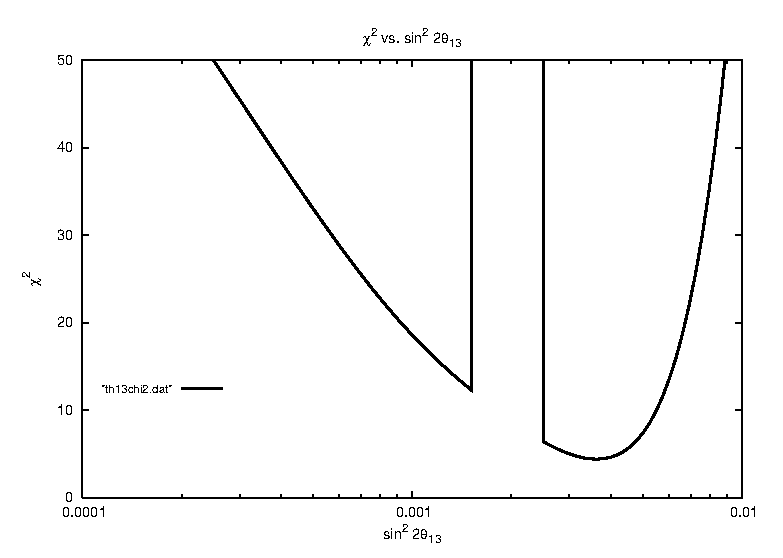
\includegraphics[height=5cm]{th13chi2-1.eps}
    \raisebox{-.5cm}{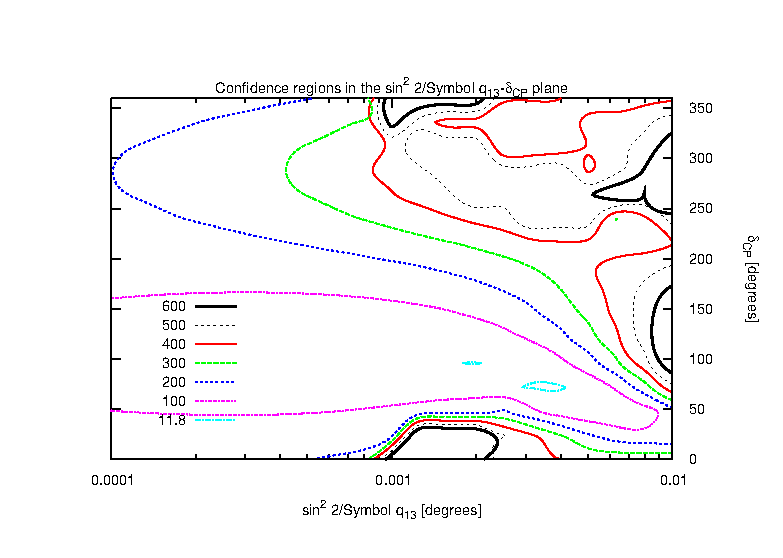
\includegraphics[height=6cm]{th13delta-NF.eps}}
  \end{center}
  \caption{Left: $\chi^2$ as a function of $\sthchooz$ for the wrong
    (inverted) hierarchy solution in a neutrino factory. Right: $\chi^2$
    contours in the $\sthchooz$--$\delta_{CP}$ plane.}
  \label{fig:th13chi2-1}
\end{figure}


\aufg{4}{Choosing better starting values}

The above discussion already suggests a solution to the degeneracy problem in
this particular case: Choose more appropriate starting values for the
minimization.  Use the function {\tt glbSetOscParams} to set $\delta_{CP}$ to
$\pi/2$ in {\tt test\_values} before calling {\tt glbChiTheta13}. The result,
shown in fig.~\ref{fig:th13chi2-2}, shows that this solves the problem in this
particular case.

\begin{figure}
  \begin{center}
    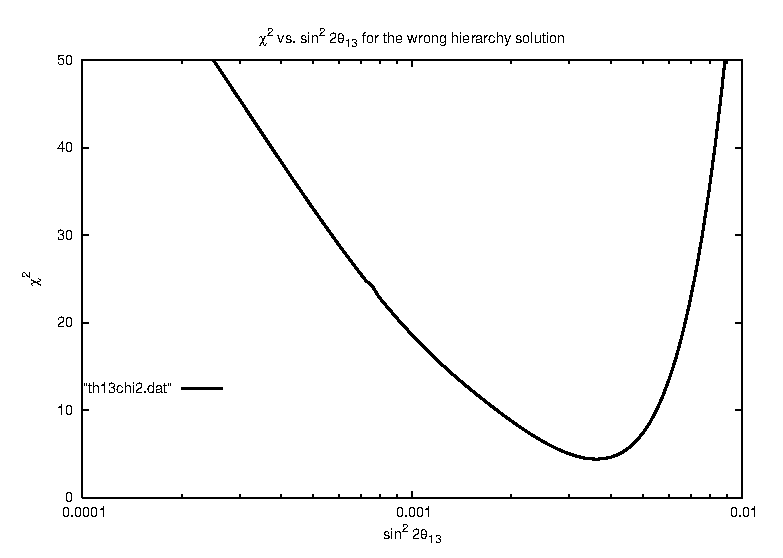
\includegraphics[height=5cm]{th13chi2-2.eps}
  \end{center}
  \caption{Solution to problems 4 and 5: The correct $\chi^2$ function for the
    wrong hierarchy solution at the neutrino factory.}
  \label{fig:th13chi2-2}
\end{figure}


\aufg{5}{A tracking algorithm}

Choosing appropriate starting values for the minimization is not a very
robust solution to the degeneracy problem. In particular, it will fail once we
choose different ``true'' parameter values, but do not adjust our starting
values. (Try choosing $\delta_{CP}^{\rm true} = \tfrac{5}{4} \pi$ to see this.)
A more robust approach is the so-called tracking algorithm: When scanning over
one parameter ($\sthchooz$ in our case), use the location of the minimum
found for one value of $\sthchooz$ as the starting point for the minimization
for the next $\sthchooz$.

To implement this algorithm, modify {\tt th13chi2.c} by allocationg an
additional parameter vector, called e.g.\ {\tt loc\_min}, and pass it to
{\tt glbChiTheta13} as its second argument. It will be filled with the location
of the minimum. In the next iteration, use {\tt loc\_min} to initialize
{\tt test\_values}. Your code should now produce a result like
fig.~\ref{fig:th13chi2-2}, but will still work when you change the ``true''
parameter values, e.g.\ to $\delta_{CP}^{\rm true} = \tfrac{5}{4} \pi$.


\aufg{6}{{\tt degfinder}, a flexible degeneracy finder using pre-scanning}

One of the most elegant solution to the problem of degeneracy finding is to
perform a quick and dirty preliminary scan of the relevant parts of parameter
space to get the rough locations of the degenerate solutions, and then use
these as starting points for local minimization. Here, quick and dirty means
that no minimization is performed over less relevant parameters (like
$\theta_{12}$ and $\sdm$), systematical errors are not taken into account, etc.
While it is straightforward to implement this algorithm, we will here use an
existing routine called {\tt degfinder}.

To use {\tt degfinder}, the following steps are necessary:
\begin{enumerate}
  \item Define the parameters that should be included in the preliminary
    scan of the parameter space, and the ranges over which you want to
    scan. In our case, we are only going to scane over $\delta_{CP}$, and
    we are going to use 8 steps (i.e.\ a step size of $\pi/4$.
    \begin{verbatim}
int n_prescan_params = 1;              /*# of params for prescan    */
int prescan_params[] = {GLB_DELTA_CP}; /*List of params to scan over*/
double prescan_min[] = {0.0         }; /*Lower edge of scan range   */
double prescan_max[] = {2*M_PI      }; /*Upper edge of scan range   */
int prescan_steps[]  = {8           }; /*Number of steps            */
    \end{verbatim}

  \item Define the {\tt glb\_projection} for the preliminary scan and
    for the finial fit. In our case, we will keep all parameters
    fixed in the prescan, and marginalize over all of them (except,
    of course, $\theta_{13}$), in the final fit.
    \begin{verbatim}
glb_projection prescan_proj = glbAllocProjection();
glbDefineProjection(prescan_proj, GLB_FIXED, GLB_FIXED, GLB_FIXED,
                                  GLB_FIXED, GLB_FIXED, GLB_FIXED);
glbSetDensityProjectionFlag(prescan_proj, GLB_FIXED, GLB_ALL);

glb_projection proj = glbAllocProjection();
glbDefineProjection(proj, GLB_FREE, GLB_FIXED, GLB_FREE,
                          GLB_FREE, GLB_FREE, GLB_FREE);
glbSetDensityProjectionFlag(proj, GLB_FREE, GLB_ALL);
    \end{verbatim}

  \item Allocate data structures where {\tt degfinder} can store the
    locations of the minima and the corresponding $\chi^2$ values.
    \begin{verbatim}
const int max_deg = 32;          /* Max # of degeneracies expected */
int n_deg;                       /* # of degeneracies found        */
double deg_chi2[max_deg];        /* chi^2 values at degeneracies   */
glb_params deg_pos[max_deg];     /* Locations of degeneracies      */
for (i=0; i < max_deg; i++)
  deg_pos[i] = glbAllocParams();
    \end{verbatim}

  \item Call {\tt degfinder} where you would normally call {\tt glbChiNP}, {\tt
    glbChiTheta13}, etc. In particular, make sure that {\tt
    glbSetCentralValues}, {\tt glbSetInputErrors} (defining external priors),
    {\tt glbSetOscillationParameters}, and {\tt glbSetRates} (computing
    ``true'' event rates) are called before any invocation of {\tt degfinder}.
    \begin{verbatim}
degfinder(test_values, n_prescan_params, prescan_params,
          prescan_min, prescan_max, prescan_steps,
          prescan_proj, proj, &n_deg, deg_pos, deg_chi2,
          DEG_NO_NH);    
    \end{verbatim}
    Besides the arguments discussed above, {\tt degfinder} accepts the
    following flags (which can be combined using binary OR):

    \begin{tabular}{lp{12cm}}
      \tt DEG\_NO\_NH    & Ignore normal hierarchy solutions in prescan. Note
                           that there is a small danger that the final minimization
                           might still converge into a normal hierarchy solution.    \\
      \tt DEG\_NO\_IH    & Ignore normal hierarchy solutions in prescan. Note
                           that there is a small danger that the final minimization
                           might still converge into an inverted hierarchy solution. \\
      \tt DEG\_NO\_SYS   & Switch off systematics in final fit. (Systematics are alway
                           off during prescan.)                                      \\
      \tt DEG\_NO\_CORR  & Switch off all parameter correlations, i.e.\ do not
                           minimize over oscillation parameters and matter density.
                           This overrides any contrary setting in {\tt prescan\_proj}
                           or {\tt proj}.
    \end{tabular}

  \item Evaluate the results from {\tt degfinder}
    \begin{verbatim}
double chi2 = 1.0e10;
for (i=0; i < n_deg; i++)
{     
  if (glbGetOscParams(deg_pos[i], GLB_DM_31) < 0.0)
  { 
    if (deg_chi2[i] < chi2)
      chi2 = deg_chi2[i];
  } 
  else
    fprintf(stderr, "Error: Minimizer converged into NH minimum."
                    "This should not have happened.\n");
}     
    \end{verbatim}

  \item Clean up
    \begin{verbatim}
for (i=0; i < max_deg; i++)
  if (deg_pos[i] != NULL)  { glbFreeParams(deg_pos[i]); deg_pos[i] = NULL; }
glbFreeProjection(proj);
glbFreeProjection(prescan_proj);    
    \end{verbatim}
\end{enumerate}

If you run the resulting program, you should again obtain a result similar to
fig.~\ref{fig:th13chi2-2}. By adding a few lines of debug output to your code,
you can easily verify that, for $\sthchooz \gtrsim 0.002$, {\tt degfinder}
indeed finds two local minima, but picks the correct one in the end.


\end{document}


